% Created 2016-03-30 Wed 10:06
\documentclass{article}
\usepackage[utf8]{inputenc}
\usepackage[T1]{fontenc}
\usepackage{fixltx2e}
\usepackage{graphicx}
\usepackage{longtable}
\usepackage{float}
\usepackage{wrapfig}
\usepackage{rotating}
\usepackage[normalem]{ulem}
\usepackage{amsmath}
\usepackage{textcomp}
\usepackage{marvosym}
\usepackage{wasysym}
\usepackage{amssymb}
\usepackage{hyperref}
\tolerance=1000
\usepackage{minted}
\usepackage{listingsutf8}
\usepackage[bottom]{footmisc} %% to keep entire footers on one page
\usepackage[]{graphicx}
\usepackage[]{minted}
\usepackage[margin=1in]{geometry}
\usepackage{comment}
\usepackage[linesnumbered,ruled,lined,shortend]{algorithm2e}
\usepackage[space]{grffile}
\setcounter{secnumdepth}{4}
\author{Nicholas Mitchell}
\date{\today}
\title{6a\_flowcharts}
\hypersetup{
  pdfkeywords={},
  pdfsubject={},
  pdfcreator={Emacs 24.5.1 (Org mode 8.2.10)}}
\begin{document}

\maketitle
\tableofcontents



\section{Appendix 1 - Flowcharts \label{flowcharts}}
\label{sec-1}


\subsection{Flowchart - Twitter mining \label{flowchart-twitter-mining}}
\label{sec-1-1}

\begin{wrapfigure}{l}{0.5\textwidth}
\centering
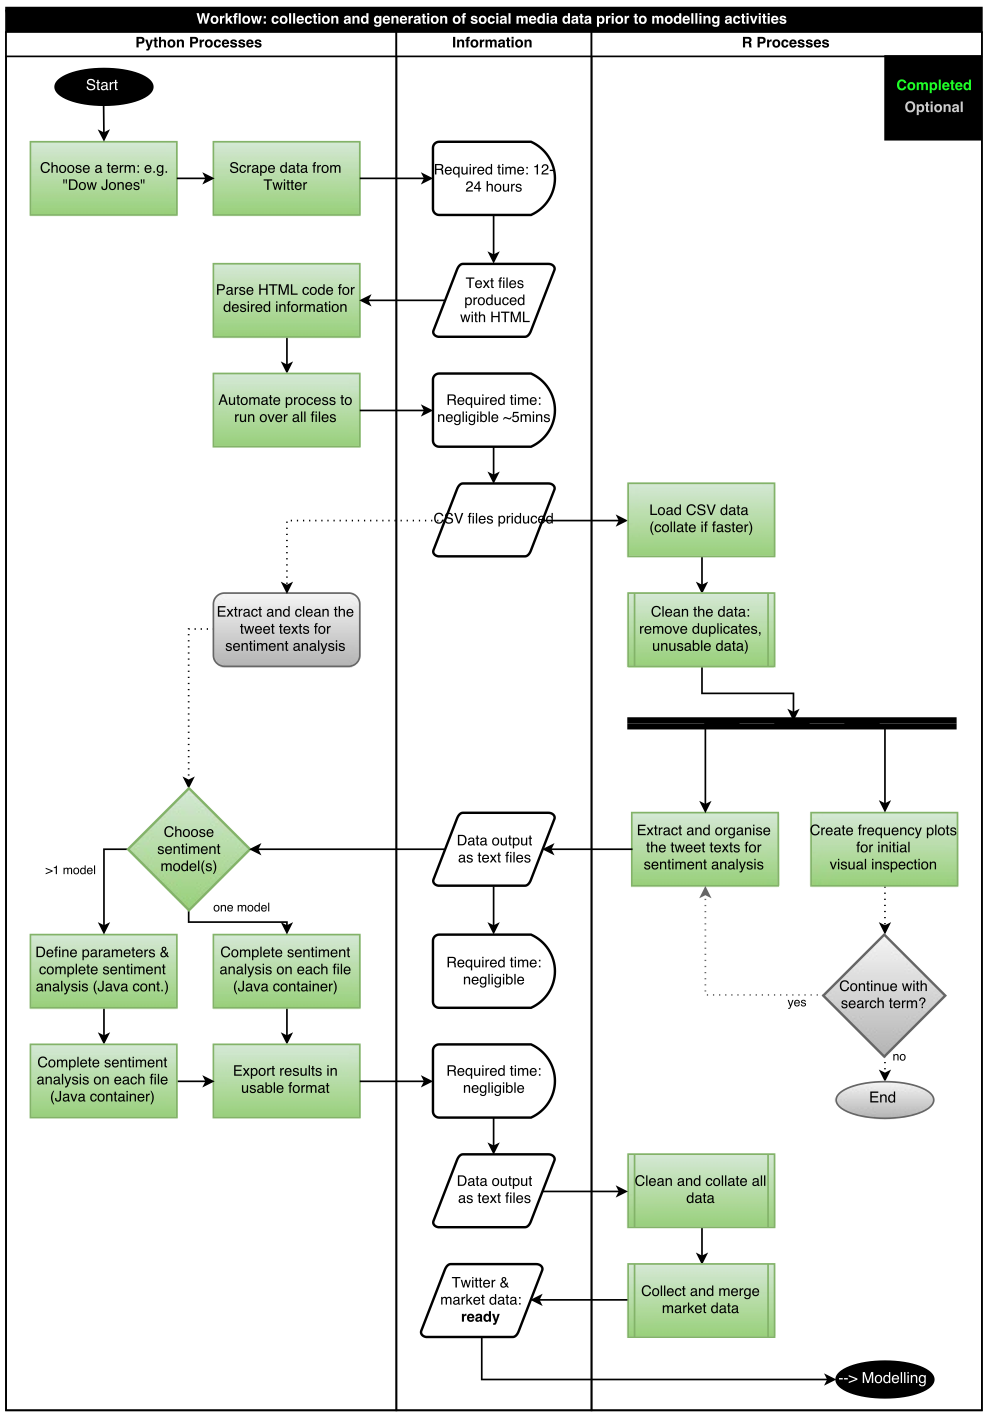
\includegraphics[width=0.48\textwidth]{/Volumes/Mac OS Drive/Thesis/Source Code/Reporting/nwm_Report/images/workflow_scraping.png}
\caption{\label{flowchart-scraping}The workflow used to scrape the Twitter Advanecd Search (TAS) interface - repeated for all thirteen search terms. The workflow has three lanes; (left) process completed using Python; (right) processees completed using R; (centre) meta-information linking various process.}
\end{wrapfigure}

\subsection{Flowchart - Modelling \label{flowchart-mod}}
\label{sec-1-2}

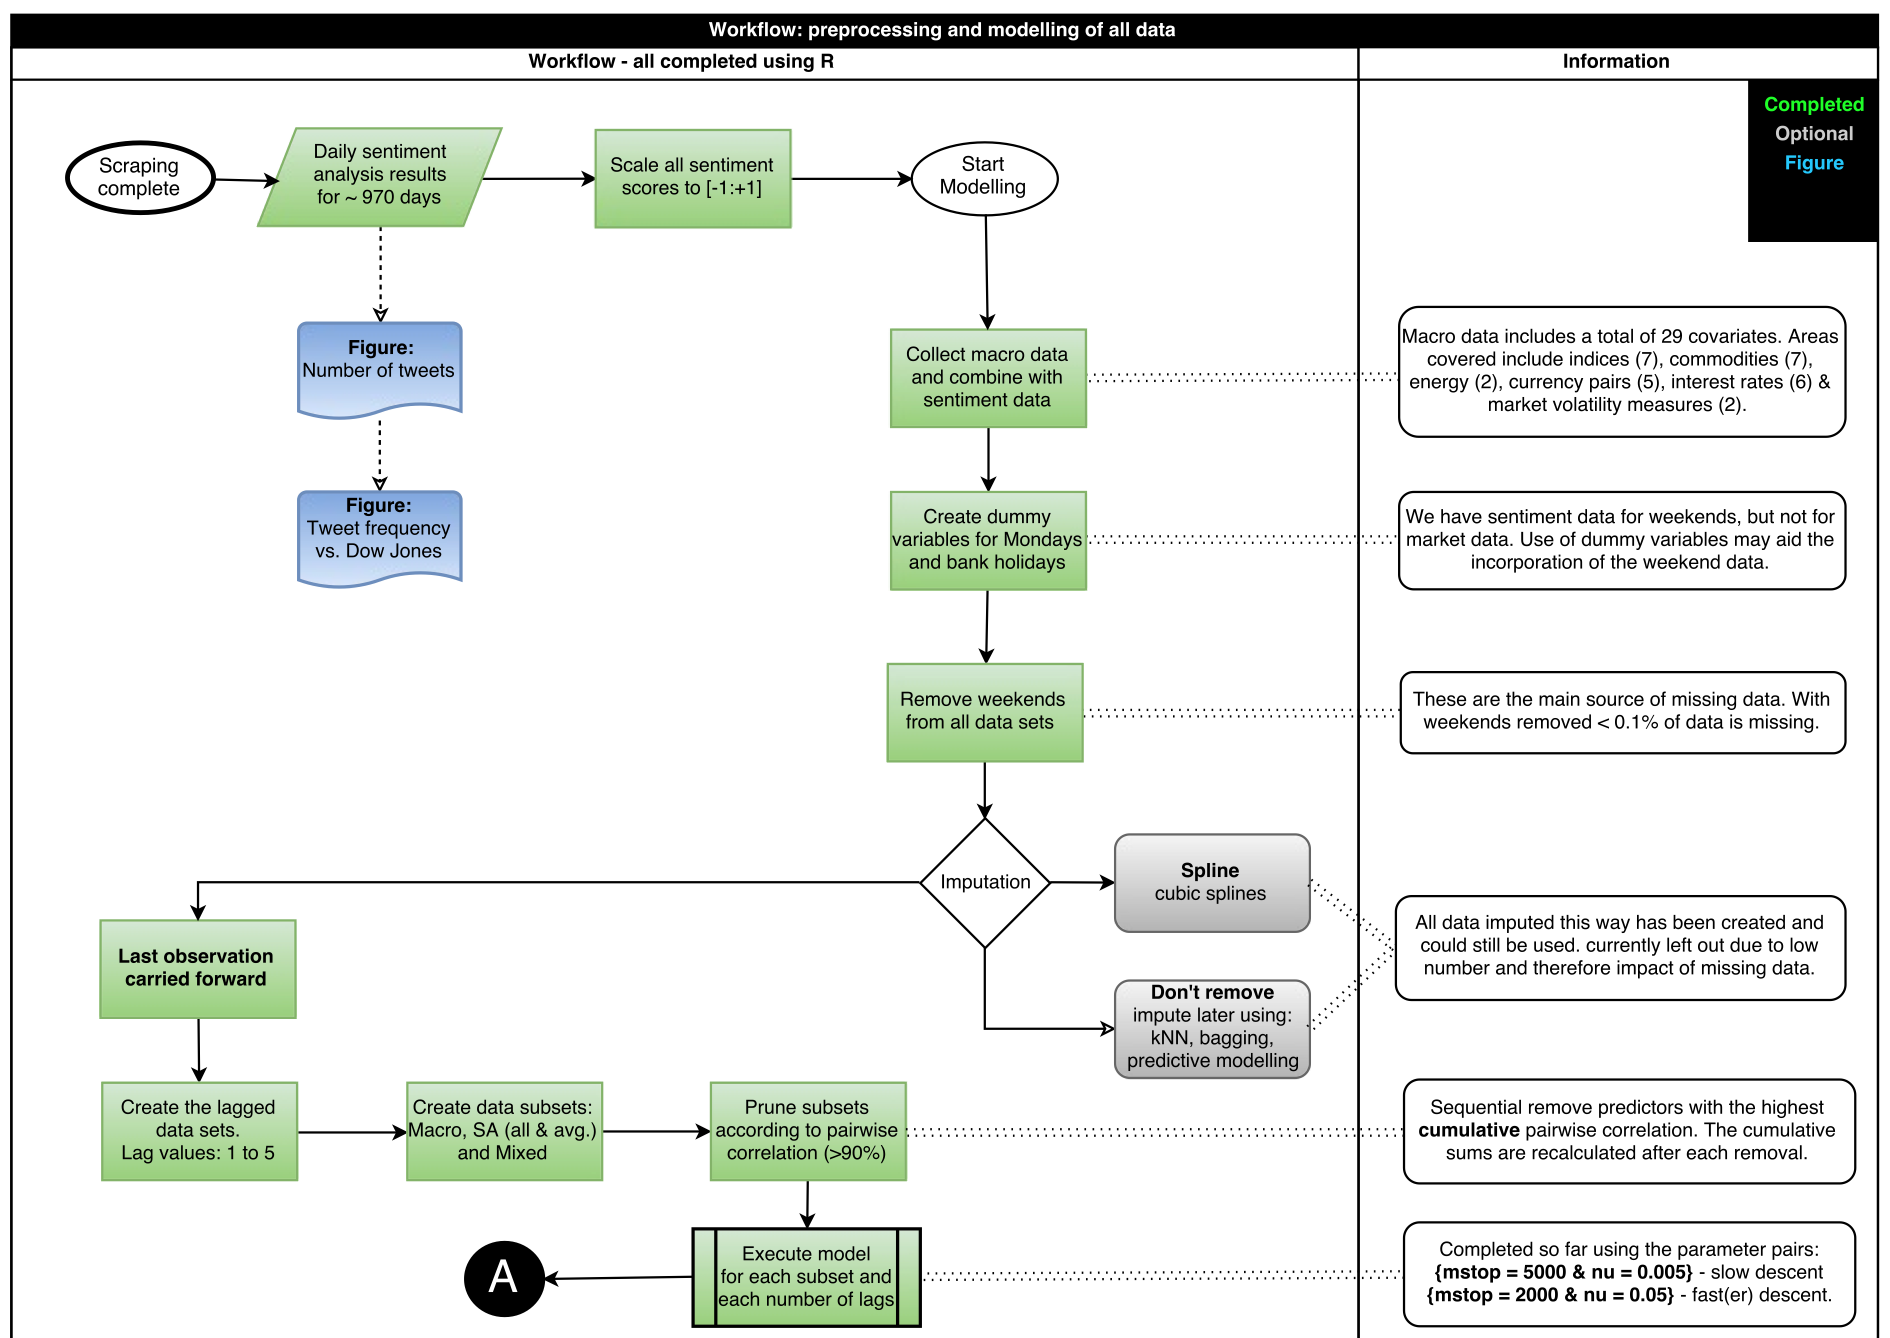
\includegraphics[angle=90,width=.9\linewidth]{/Volumes/Mac OS Drive/Thesis/Source Code/Reporting/nwm_Report/images/workflow_modelling_1.png}

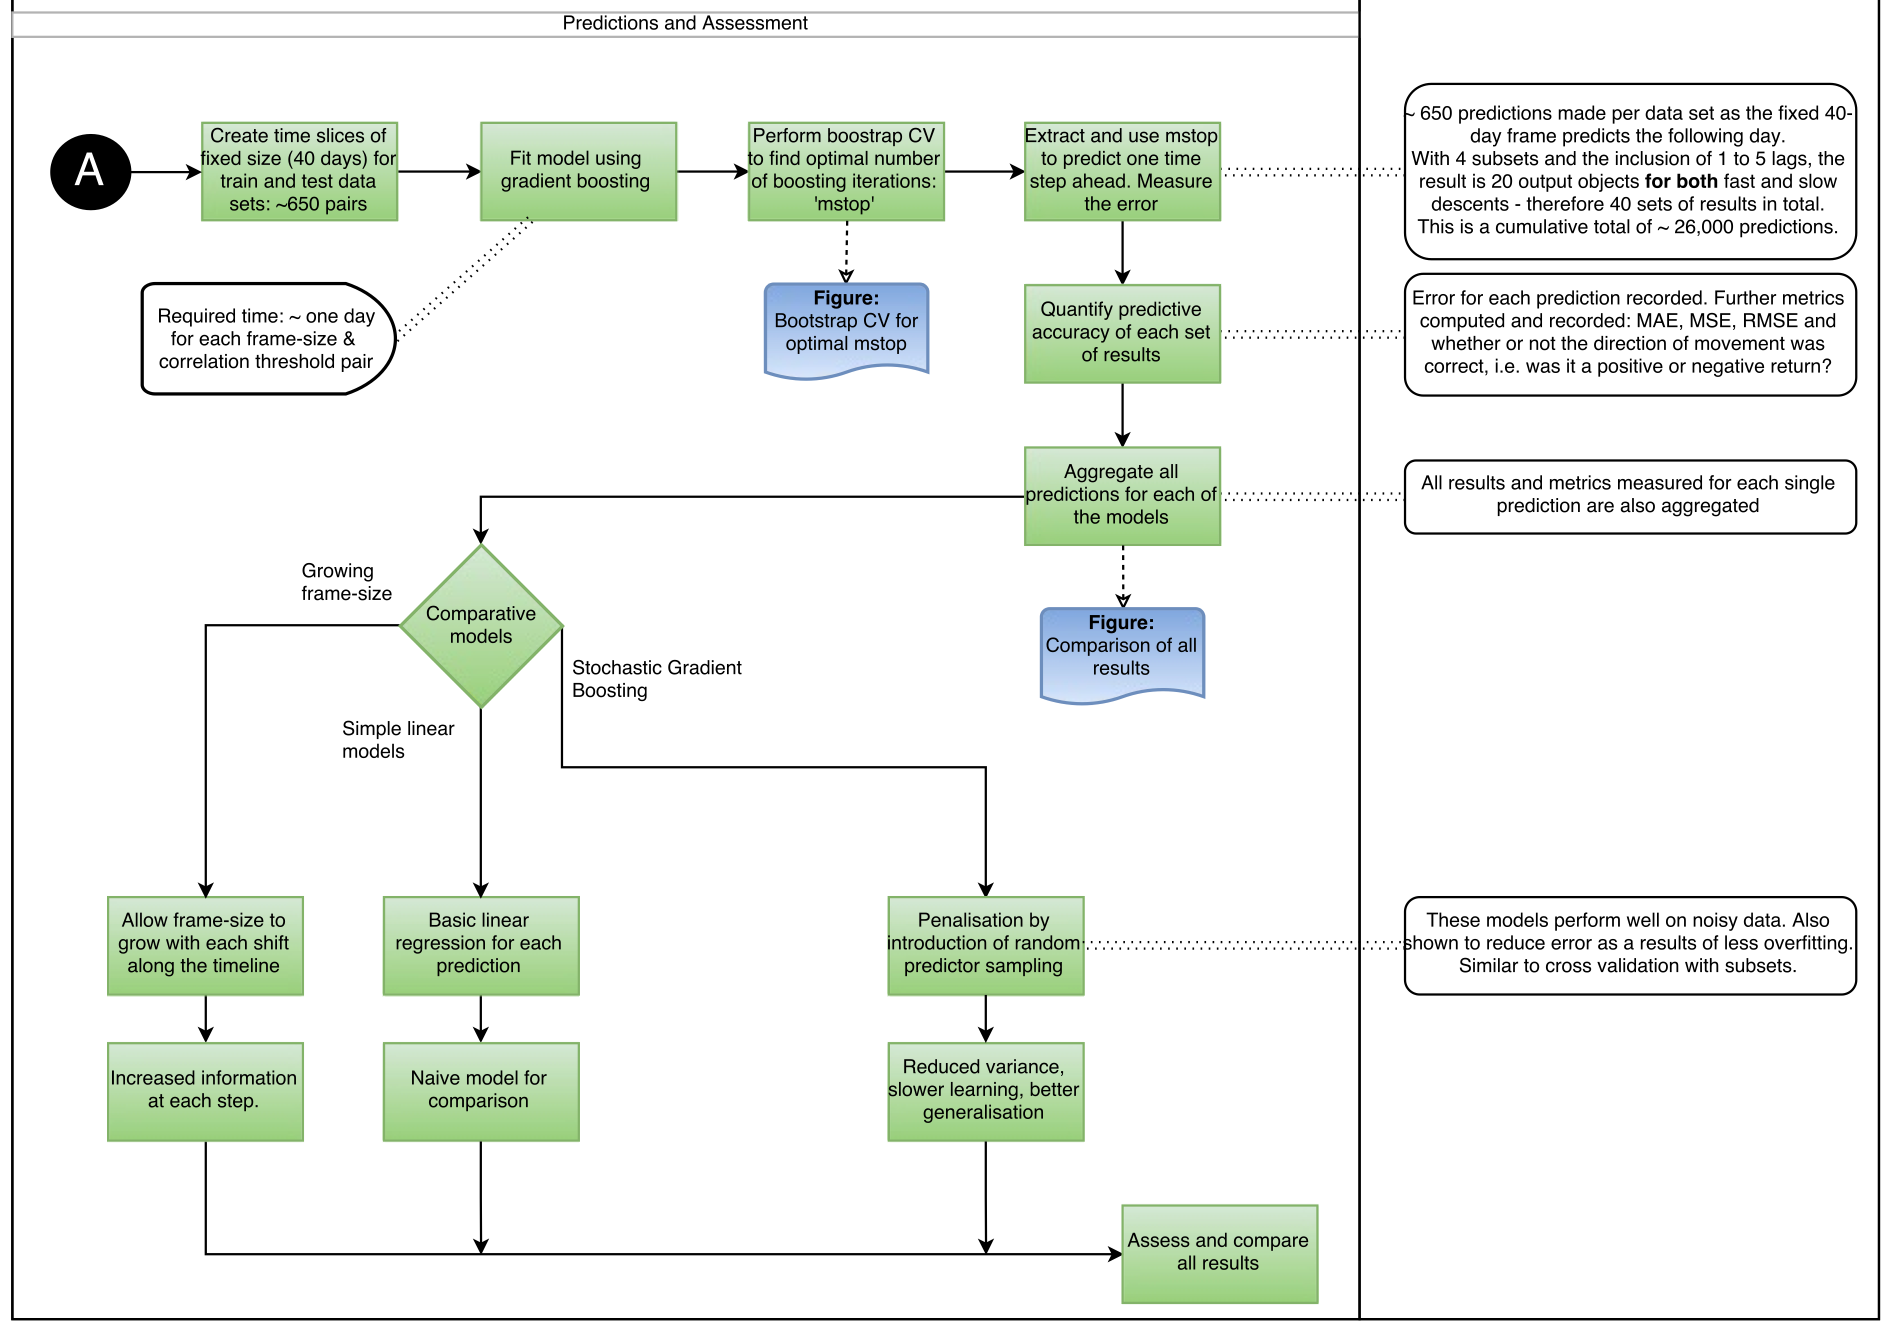
\includegraphics[angle=90,width=.9\linewidth]{/Volumes/Mac OS Drive/Thesis/Source Code/Reporting/nwm_Report/images/workflow_modelling_2.png}

\pagebreak
% Emacs 24.5.1 (Org mode 8.2.10)
\end{document}